\clearpage
\VerdierPhysicalPageAnchor{0133}%
\begingroup
\small
\setlength{\emergencystretch}{1.5em}%
\setlength{\abovedisplayskip}{1pt plus 1pt minus 1pt}%
\setlength{\belowdisplayskip}{1pt plus 1pt minus 1pt}%
\newcommand{\VerdierHatchTriangle}[3]{%
  \begin{scope}
    \clip (#1) -- (#2) -- (#3) -- cycle;
    \draw[step=.20cm,black!78,line width=.16pt] (-2,-2) grid (7,2);
  \end{scope}}

\VerdierSemanticAnchor{ch2-2-1-13}
\noindent\textbf{2.1.13.}\quad
\VerdierSemanticAnchor{ch2-2-1-13-saturation-direction}%
\emph{Si la catégorie $\mathcal D'$ est saturée, l'ensemble
$S(\mathcal D')$ est saturé.}
\VerdierSemanticAnchor{ch2-2-1-13-composable-setup}%
Soient $f,g,h$ trois morphismes composables tels que $fg$ et $gh$ soient des
éléments de $S(\mathcal D')$.

\VerdierSemanticAnchor{ch2-2-1-13-triv-construction}
Utilisant l'axiome TRIV, on peut construire un diagramme :

\VerdierSemanticAnchor{ch2-2-1-13-triv-diagram}
\begin{center}
  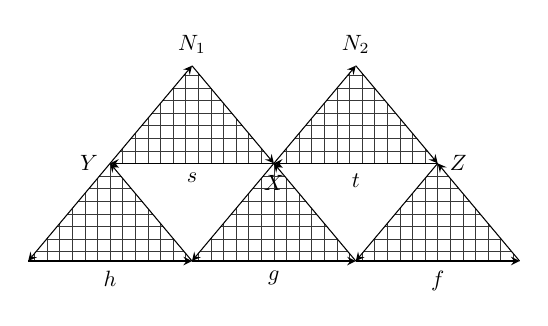
\begin{tikzpicture}[>=stealth,line width=.38pt,scale=.80,transform shape]
    \coordinate (Y)  at (0,0);
    \coordinate (X)  at (2.6,0);
    \coordinate (Z)  at (5.2,0);
    \coordinate (N1) at (1.3,1.55);
    \coordinate (N2) at (3.9,1.55);
    \coordinate (A)  at (-1.3,-1.55);
    \coordinate (Q1) at (1.3,-1.55);
    \coordinate (Q2) at (3.9,-1.55);
    \coordinate (B)  at (6.5,-1.55);

    \VerdierHatchTriangle{Y}{N1}{X}
    \VerdierHatchTriangle{X}{N2}{Z}
    \VerdierHatchTriangle{Y}{A}{Q1}
    \VerdierHatchTriangle{X}{Q1}{Q2}
    \VerdierHatchTriangle{Z}{Q2}{B}

    \draw[->] (Y) -- (N1);
    \draw[->] (N1) -- (X);
    \draw[->] (X) -- node[below=1pt] {$s$} (Y);
    \draw[->] (X) -- (N2);
    \draw[->] (N2) -- (Z);
    \draw[->] (Z) -- node[below=1pt] {$t$} (X);

    \draw[->] (Y) -- (A);
    \draw[->] (A) -- node[below=1pt] {$h$} (Q1);
    \draw[->] (Q1) -- (Y);
    \draw[->] (X) -- (Q1);
    \draw[->] (Q1) -- node[below=1pt] {$g$} (Q2);
    \draw[->] (Q2) -- (X);
    \draw[->] (Z) -- (Q2);
    \draw[->] (Q2) -- node[below=1pt] {$f$} (B);
    \draw[->] (B) -- (Z);

    \node[left=2pt]  at (Y)  {$Y$};
    \node[below=2pt] at (X)  {$X$};
    \node[right=2pt] at (Z)  {$Z$};
    \node[above=2pt] at (N1) {$N_1$};
    \node[above=2pt] at (N2) {$N_2$};
  \end{tikzpicture}
  \quad ,
\end{center}

\VerdierSemanticAnchor{ch2-2-1-13-diagram-interpretation}
\noindent où $N_1$ et $N_2$ sont des objets de $\mathcal D'$, où les cinq
triangles hachurés sont des triangles distingués et où les deux triangles
non hachurés sont commutatifs.

\VerdierSemanticAnchor{ch2-2-1-13-shifted-zero}
On en déduit que $s[1]t=0$ (1.2.2).
\VerdierSemanticAnchor{ch2-2-1-13-shifted-membership}%
De plus, en vertu de SM1) et SM5), le
morphisme $s[1]t$ est un élément de $S(\mathcal D')$.

\VerdierSemanticAnchor{ch2-2-1-13-split-triangle}
Il existe donc un triangle distingué du type $(Z,Y[2],N,0,u,v)$, où $N$ est
un objet de $\mathcal D'$.
\VerdierSemanticAnchor{ch2-2-1-13-direct-summand}%
On en déduit, en utilisant (1.2.6) et TRII, que $Y$ est facteur direct d'un
objet de $\mathcal D'$.
\VerdierSemanticAnchor{ch2-2-1-13-y-in-dprime}%
Par suite, $Y$ est
isomorphe à un objet de $\mathcal D'$.

\VerdierSemanticAnchor{ch2-2-1-13-s-triangle}
On en déduit, en utilisant (1.2.4), le fait que $\mathcal D'$ soit une
sous-catégorie triangulée de $\mathcal D$ et le triangle distingué :

\begin{center}
  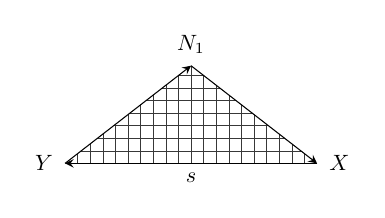
\begin{tikzpicture}[>=stealth,line width=.38pt,scale=.80,transform shape]
    \coordinate (Y)  at (-2,0);
    \coordinate (X)  at (2,0);
    \coordinate (N1) at (0,1.55);
    \VerdierHatchTriangle{Y}{N1}{X}
    \draw[->] (Y) -- (N1);
    \draw[->] (N1) -- (X);
    \draw[->] (X) -- node[below=1pt] {$s$} (Y);
    \node[left=2pt]  at (Y)  {$Y$};
    \node[right=2pt] at (X)  {$X$};
    \node[above=2pt] at (N1) {$N_1$};
  \end{tikzpicture}
\end{center}

\VerdierSemanticAnchor{ch2-2-1-13-g-membership}
\noindent que $X$ est isomorphe à un objet de $\mathcal D'$. Par suite, le
morphisme $g$ est un élément de $S(\mathcal D')$.

\VerdierSemanticAnchor{ch2-2-1-14}
\medskip
\noindent\textbf{2.1.14.}\quad
\VerdierSemanticAnchor{ch2-2-1-14-saturation-direction}%
\emph{Si l'ensemble $S(\mathcal D')$ est saturé, la sous-catégorie
$\mathcal D'$ est saturée.}

\VerdierSemanticAnchor{ch2-2-1-14-direct-summand-setup}
Soit $X$ un facteur direct d'un objet de $\mathcal D'$.
\VerdierSemanticAnchor{ch2-2-1-14-first-triangle}%
En utilisant (1.2.6)
et TRII, on voit qu'il existe un triangle distingué $(X,Y,N,0,u,v)$, où $N$
est un objet de $\mathcal D'$.
\VerdierSemanticAnchor{ch2-2-1-14-zero-morphism}%
Par suite, le morphisme nul $X\to Y$ est un
morphisme de $S(\mathcal D')$.

\VerdierSemanticAnchor{ch2-2-1-14-sm4-application}
Appliquons alors la propriété SM4) aux trois morphismes
$0\to X\to 0\to Y$.
\VerdierSemanticAnchor{ch2-2-1-14-x-zero-membership}%
On en déduit que le morphisme $X\to 0$ est un élément
de $S(\mathcal D')$.

\VerdierSemanticAnchor{ch2-2-1-14-second-triangle}
Il existe donc un triangle distingué $(X,0,N,0,0,i)$, où $N$ est un objet de
$\mathcal D'$.
\VerdierSemanticAnchor{ch2-2-1-14-shift-isomorphism}%
Par suite, le morphisme $N\xrightarrow{i}X[1]$ est un
isomorphisme. On en déduit que $X$ est isomorphe à $N[-1]$, qui est un objet
de $\mathcal D'$.

\VerdierSemanticAnchor{ch2-2-1-14-proposition-complete}
Ceci achève la preuve de la proposition (2.1.8).

\VerdierSemanticAnchor{ch2-2-1-14-p134-boundary}
\endgroup
